\documentclass{beamer}
\usepackage[english]{babel}
\usepackage[utf8]{inputenc}

\usepackage{color}
\usepackage{graphicx}
\usepackage{fancybox}


% for tick marks
%\usepackage{dingbat}

\usepackage{beamerthemesplit}
\usetheme[compress]{MPIjast}

% for recurring outline - if check
% source: http://tex.stackexchange.com/a/26039
\usepackage{etoolbox}


\title[Toponym Resolution and Adaptive Context Features]{Toponym Resolution and Adaptive Context Features}
\subtitle{}
\author[Faraz Ahmad]{Faraz Ahmad}
\date{\today}
\institute[MPI-Inf]{
Max Planck Institute for Informatics\\
Saarland Informatics Campus\\
\color{MPIIblue}{s8faahma@stud.uni-saarland.de}}

%---------------------------------------%
%---------- RECURRING OUTLINE ----------%
% have this if you'd like a recurring outline
\AtBeginSection[]  % "Beamer, do the following at the start of every section"
{
	\ifnumcomp{\value{section}}{=}{1}{}
	{
		\begin{frame}[t]
			\frametitle{Outline}
			\tableofcontents[sectionstyle=show/shaded,hideallsubsections]
		\end{frame}
	}
} 
{
%\begin{frame}<beamer> 
%\frametitle{Outline} % make a frame titled "Outline"
%\tableofcontents[currentsection,hideallsubsections]  % show TOC and highlight current section
%\end{frame}
%}
%----------------------------------------


\begin{document}
\frame[plain]{\titlepage}
%\frame{\frametitle{Outline}\tableofcontents[hideallsubsections]}

%========================================
%========================================

\section[Motivation]{Motivation}

%###############################################

%###############################################

%----------------------------------------


%\subsection{Terminology}
%
%\frame{
%\frametitle{Terminology}
%
%\begin{itemize}
%\item Toponyms
%\item Geotagging
%\begin{itemize}
%	\item Toponym recognition
%	\item Toponym disambiguation
%\end{itemize}
%\item Difficulty in Geotagging
%\item Gazeteers
%\end{itemize}
%} % END OF FRAME

%----------------------------------------

\subsection{Toponyms}
\frame{
\frametitle{Toponyms}
\begin{block}{Toponyms}
	Words in a document text that correspond to \textbf{location names} are called toponyms.
\end{block}

refer to a \textbf{populated place}, such as:\\
\begin{itemize}
	\item Cities/Towns
	\item States/Provinces
	\item Countries
\end{itemize}


} % END OF FRAME

%----------------------------------------

\frame[t]{
\frametitle{Toponyms - examples}

\begin{block}{Toponyms examples: }
	\begin{itemize}
		\item[(1)]  ``\underline{\textbf{France}} won the world cup in 1998."
		\pause
		\item[(2)] ``\underline{\textbf{Birmingham}}, a major city of \underline{\textbf{West Midlands}} is the second most populous city of \underline{\textbf{England}}, third most populous is \underline{\textbf{Leeds}}."
		\pause
	\end{itemize}
\end{block}

\begin{columns}
	\begin{column}{.5\textwidth}
		\begin{figure}
			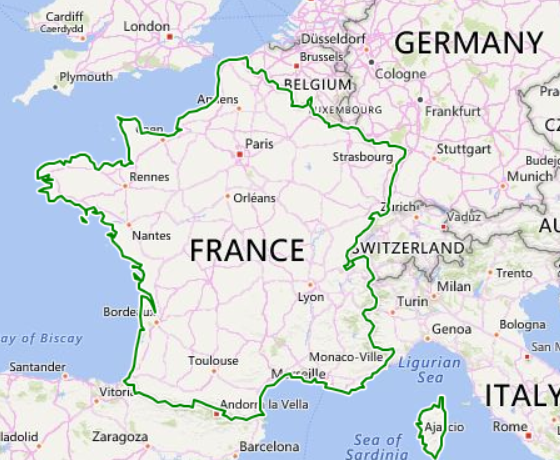
\includegraphics[width=\textwidth]{france.png} 
			%\caption{AvH in Wikipedia, \textit{Source: URL}}
		\end{figure}
	\end{column}
	\begin{column}{.5\textwidth}
		\begin{figure}
			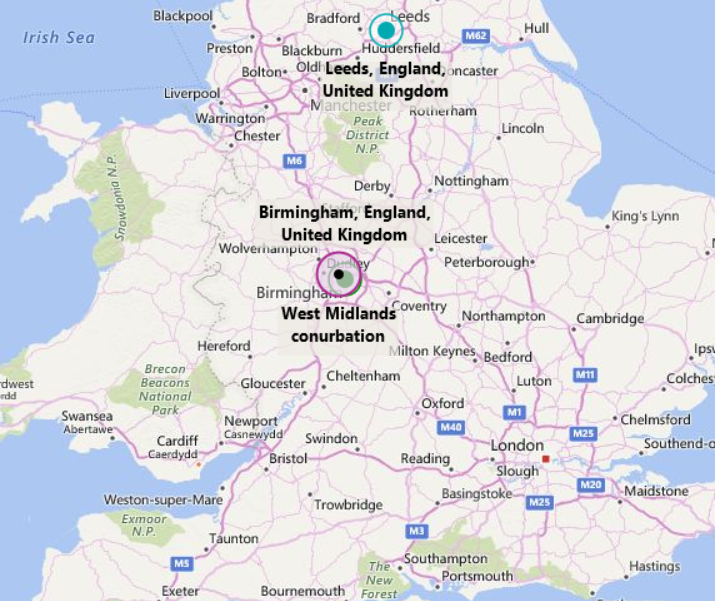
\includegraphics[width=\textwidth]{uk.png} 
			%\caption{AvH in Wikipedia, \textit{Source: URL}}
		\end{figure}
	\end{column}
	
\end{columns}

\vfill
} % END OF FRAME

%========================================

\subsection{Geotagging}


\frame{
\frametitle{Geotagging}

\begin{block}{Geotagging}
	understanding the {geographic content} of a text document.
\end{block}

is a two step process:\\
\begin{itemize}
	\item[(1)] detecting the toponyms
	\item[(2)] grounding the detected toponyms
\end{itemize}

\vfill
} % END OF FRAME

%----------------------------------------

\frame{
\frametitle{Geotagging - example}
\begin{block}{sentence }
	``France won the world cup in 1998."
\end{block}
\pause
\begin{block}{step 1: detecting the toponyms = Toponym recognition}
	``\underline{France} won the world cup in 1998."
\end{block}
\pause
\begin{block}{step 2: grounding the detected toponyms = Toponym resolution}
``\underline{France} (lat 46, long 2) won the world cup in 1998."
\end{block}

\vfill
} % END OF FRAME

%----------------------------------------

%\frame{
%	\frametitle{Geotagging - the two steps defined}
%	
%	\begin{itemize}
%		\item Toponym recognition (Geoparsing)
%		\item Toponym resolution (Geocoding)
%	\end{itemize}
%	 
%	 
%	\begin{block}{Toponym recognition}
%		\textbf{detect} all the \textbf{toponyms} (location
%		names) in text.
%	\end{block}
%	\begin{block}{Toponym resolution}
%		\textbf{assign} the \textbf{correct lat/long value} to \textbf{toponyms}.
%	\end{block}
%	
%	\vfill
%} % END OF FRAME
%
%%----------------------------------------
%
%\frame{
%	\frametitle{Geotagging - example}
%	\begin{block}{sentence }
%		``France won the world cup in 1998."
%	\end{block}
%	\begin{block}{step 1: detecting the toponyms = Toponym recognition}
%		``\underline{France} won the world cup in 1998."
%	\end{block}
%	\begin{block}{step 2: grounding the detected toponyms = Toponym resolution}
%		``\underline{France} (lat 46, long 2) won the world cup in 1998."
%	\end{block}
%	
%	\vfill
%} % END OF FRAME

%========================================

%\subsection{Difficulty in Geotagging}
%
%
%\frame{
%\frametitle{Difficulty in Geotagging}
%
%\begin{block}{in toponym recognition}
%	need to understand natural language in order to detect toponyms accurately.
%\end{block}
%
%\begin{block}{in toponym resolution}
%	need to understand document's content to ground a toponym to its correct lat/long value \textbf{(correct interpretation)}.
%\end{block}
%
%
%} % END OF FRAME

\subsection{Difficulty in Geotagging}


\frame{
	\frametitle{Difficulty in Geotagging - ambiguity}
	
	\begin{itemize}
		\item geo/geo ambiguity
		\item geo/non-geo ambiguity
	\end{itemize}

	\pause
	
	\begin{block}{geo/geo ambiguity}
		\textbf{"Hyderabad"}, it is a city in Pakistan and India.
	\end{block}
	
	\pause
	
	\begin{block}{geo/non-geo ambiguity}
		\textbf{"Jordan"}, it is a name of a country and a person
	\end{block}
	
	
} % END OF FRAME
%========================================

\subsection{Gazeteers}


\frame{
	\frametitle{Gazeteers}
	
	\begin{block}{Gazeteer}
		look up table for looking up toponyms and getting their features
	\end{block}

	get features of toponyms interpretations:
	\begin{itemize}
		\item population
		\item no. of interpretations
		\item alternative names
		\item location type
		\item \textbf{lat/long value} for each interpretation
	\end{itemize}
	
} % END OF FRAME

%----------------------------------------

\frame{
	\frametitle{Gazeteers}
	
	some examples of online available gazeteers
	\begin{itemize}
		\item GeoNames
		\item World Factbook by CIA
	\end{itemize}
	
	\begin{figure}
		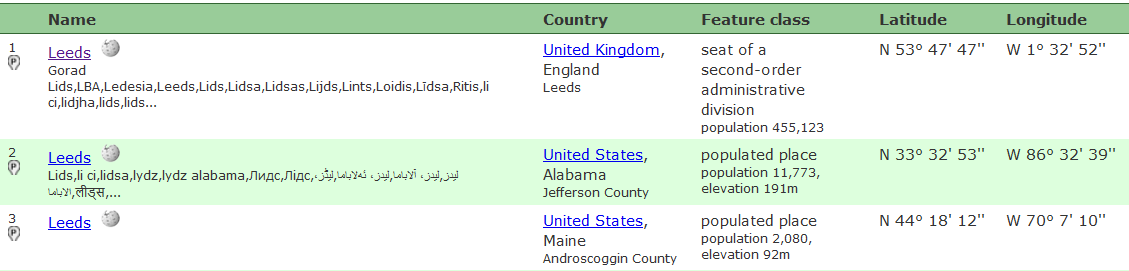
\includegraphics[width=\textwidth]{geonames.png} 
		\caption{GeoNames gazeteer}
	\end{figure}
		
} % END OF FRAME

%========================================
%========================================

%\section[Motivation1]{Motivation1}


\subsection{Geographic content in queries}

\frame{
	\frametitle{Geographic content in queries}
	
	\begin{itemize}
		\item 14.8\% geographic queries in 2001 Excite search engine log
		\item 13\% geographic queries (related to USA) in 3 months data of AOL search engine in 2006 
	\end{itemize}
	
	
} % END OF FRAME

%----------------------------------------


%========================================
%========================================



\subsection{NERD vs Geotagging}


\frame{
\frametitle{NERD vs Geotagging}

\begin{table}[bt]
	\begin{tabular}{|c|c|} \hline
		\textbf{NERD}      & \textbf{Geotagging} \\ 
		\hline
		\uncover<2->{NER more general} & \uncover<2->{specific to locations} \\
		\uncover<3->{named entities} & \uncover<3->{only toponyms} \\
		\uncover<4->{low recognition recall} & \uncover<4->{higher recognition recall} \\
		\hline
		\uncover<5->{knowledge bases} & \uncover<5->{gazeteers} \\
		\uncover<6->{ground = link} & \uncover<6->{ground = lat/long} \\
		\uncover<7->{knowledgebases are general}  & \uncover<7->{gazeteers are specific} \\ 
		\hline
	\end{tabular}
\end{table}

%\begin{columns}
%	\begin{column}{.5\textwidth}
%			\alert{NERD}
%			\begin{itemize}
%				\item disambiguate all entities
%				\item uses knowledgebases to ground entities
%				\item ground = link to the correct knowledgebase entry about entity
%				\item knowledgebases are more general
%			\end{itemize}
%	\end{column}
%	\begin{column}{.5\textwidth}
%			\alert{Geotagging}
%			\begin{itemize}
%				\item disambiguate only toponyms
%				\item uses various features to ground toponyms
%				\item ground = assign correct lat/long value to the toponym
%				\item gazeteers are more geographically focussed
%				\item gazeteers have many toponyms
%			\end{itemize}
%	\end{column}
%\end{columns}

%\pause

%\begin{block}{Bottom line}
%	Geotagging deserves attention in its own right, and NERD cannot be used for it.
%\end{block}

\vfill
} % END OF FRAME

%----------------------------------------
\subsection{NERD for doing Geotagging?}


\frame{
	\frametitle{NERD for doing Geotagging?}
	
	\begin{overprint}
		\onslide<1>
		\begin{figure}
			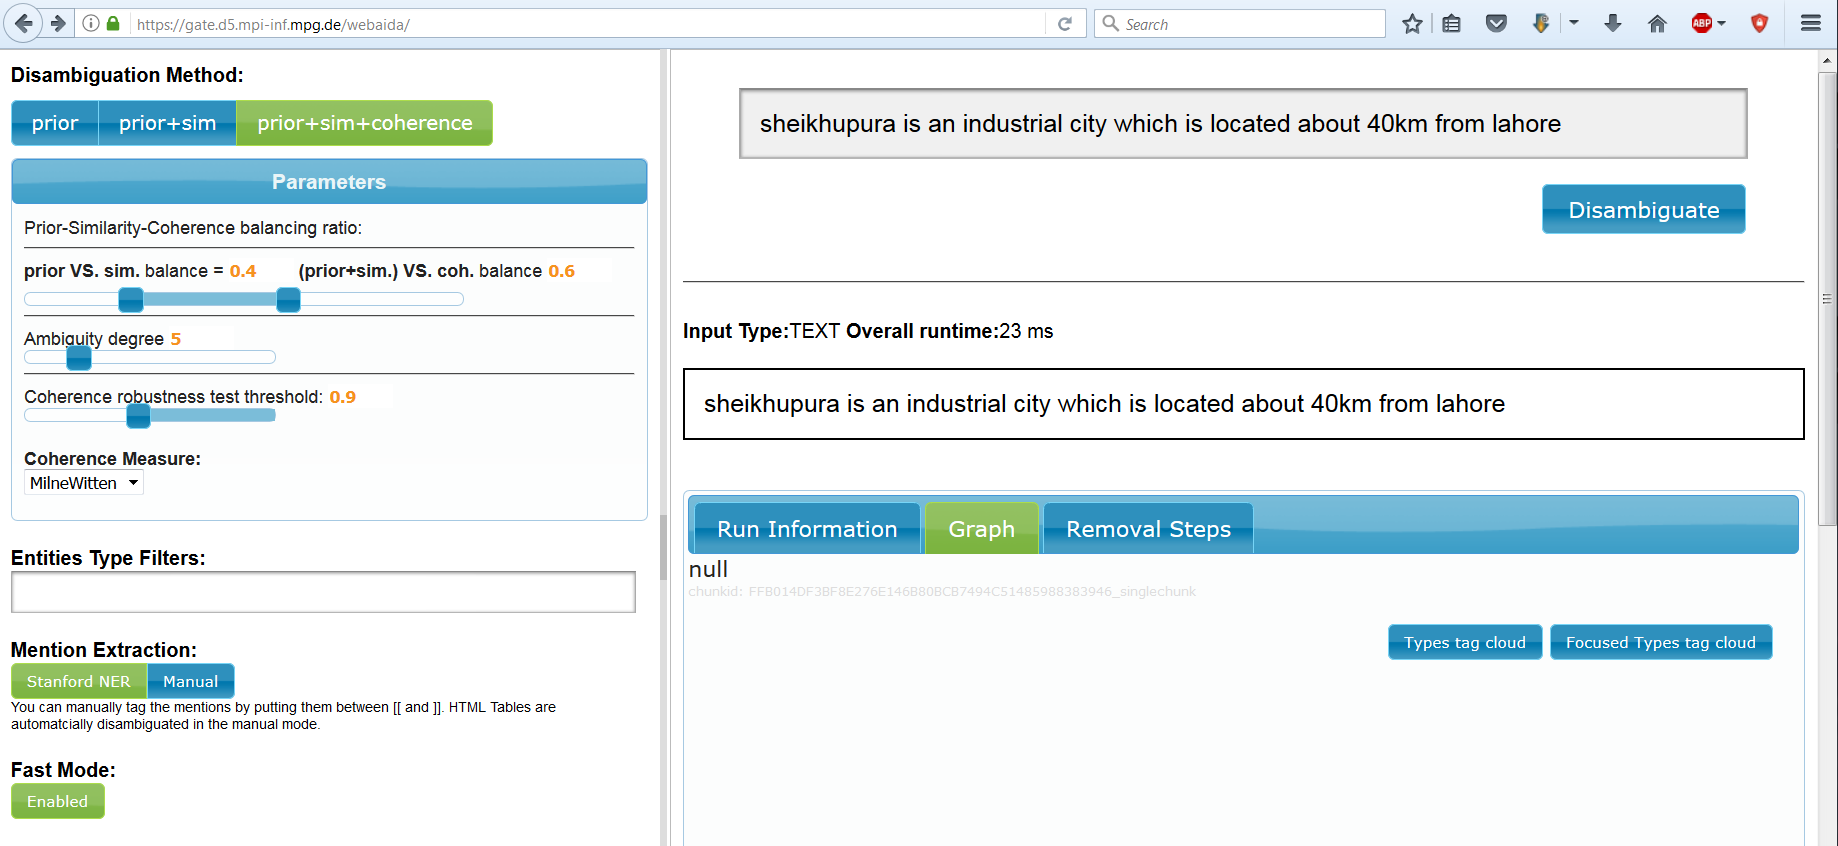
\includegraphics[width=\textwidth]{aida.png} 
			\caption{from AIDA Web Interface, \textit{Source: URL}}
		\end{figure}
		
		\onslide<2>
		\begin{figure}
			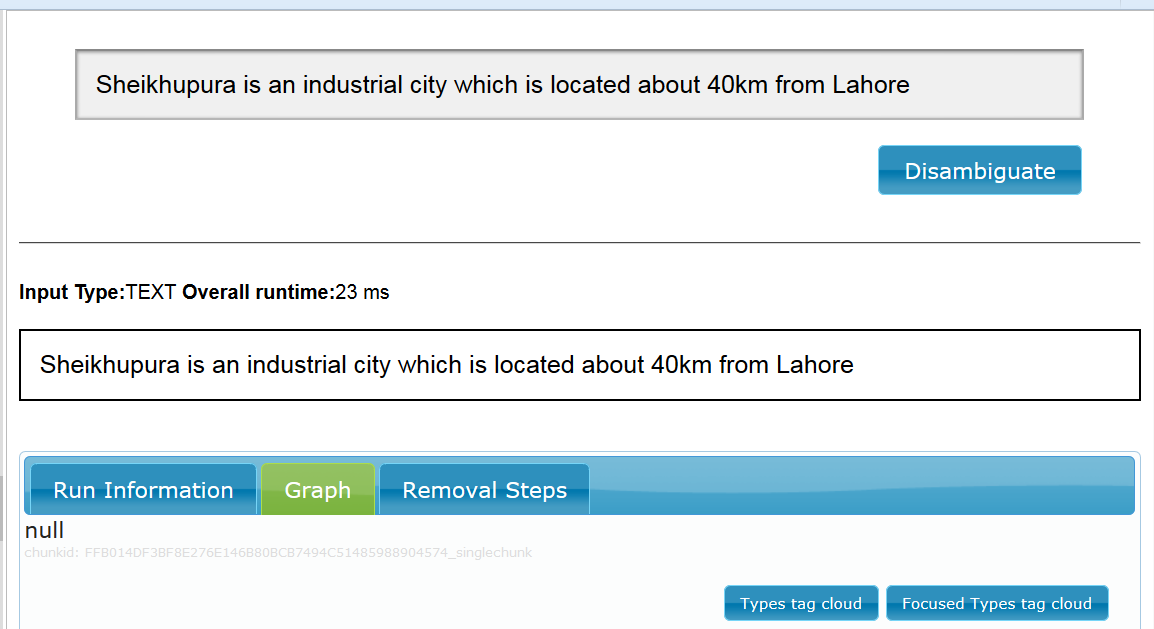
\includegraphics[width=\textwidth]{aida1.png} 
			\caption{from AIDA Web Interface, \textit{Source: URL}}
		\end{figure}
	
		\onslide<3>
		\begin{figure}
			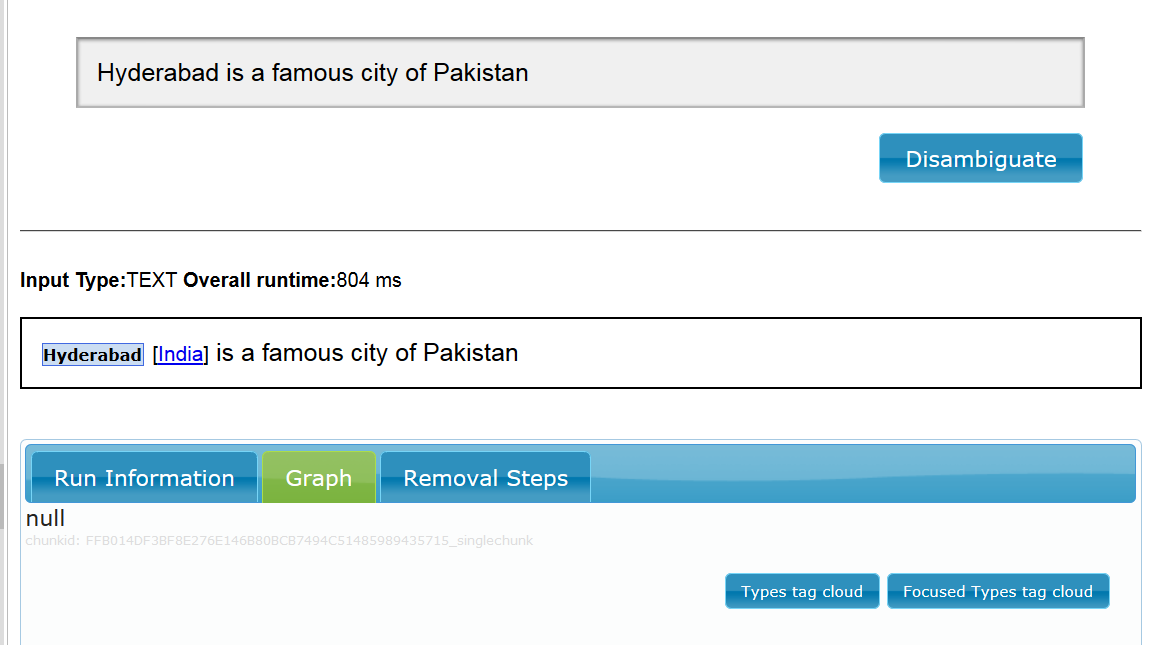
\includegraphics[width=\textwidth]{aida2.png} 
			\caption{from AIDA Web Interface, \textit{Source: URL}}
		\end{figure}
	
		\onslide<4>
		\begin{figure}
			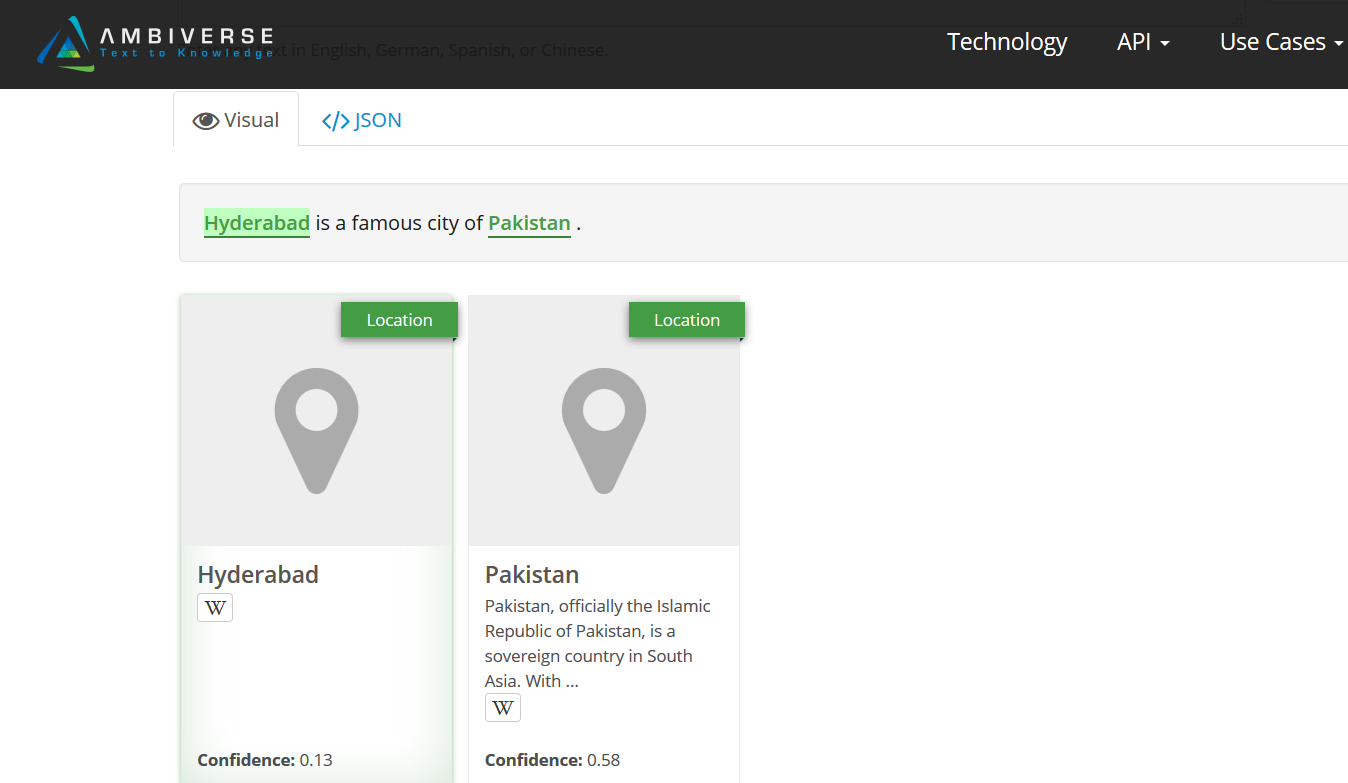
\includegraphics[width=\textwidth]{ambi.png} 
			\caption{from Ambiverse Entity Linking Demo, \textit{Source: URL}}
		\end{figure}
	
	\end{overprint}
	
	\vfill
} % END OF FRAME

%----------------------------------------
%========================================


\section[Adaptive Context Features]{Adaptive Context Features}

\subsection{Toponym recognition procedure}
\frame{
	\frametitle{Toponym recognition procedure}
	
	\begin{itemize}
		\item multi-faceted recognition
		\item tokenization
		\item lookups
		\item statistical NLP tools (NER)
		\item POS tagging
		\item has high recall!
\end{itemize}
} % END OF FRAME
%----------------------------------------

\subsection{Toponym resolution procedure}
\frame{
	\frametitle{Toponym resolution procedure}
	
	\begin{itemize}
		\item cast as classification problem
		\item identify each toponym/interpretation pair as correct or incorrect
		\item used decision trees
		\item can get confidence score for each decision
		\item restores precision!
	\end{itemize}
\vfill
} % END OF FRAME
%----------------------------------------

\subsection{Input features }
\frame{
	\frametitle{Input features for resolution}
	
	\begin{itemize}
		\item Context free features
		\item Adaptive context features
	\end{itemize}

	\pause

	\begin{block}{Context free features}
		 do not depend on the context (window) of the toponym t being resolved; usually available from gazeteers
	\end{block}

	\pause
	
	\begin{block}{Adaptive context features}
		depend on the context (window) around the toponym t being resolved; other toponyms in the window	around toponym t help in resolving it
	\end{block}
\vfill
} % END OF FRAME
%----------------------------------------

\subsection{Context Free Features}
\frame{
	\frametitle{Context Free Features}
	
	\begin{columns}
		\begin{column}{.3\textwidth}
				\begin{itemize}
				\item Interpretations
				\item Population
				\item Altnames
				\item Dateline
				\item Locallex
			\end{itemize}
		\end{column}
		\begin{column}{.7\textwidth}
			\pause
			\begin{figure}
				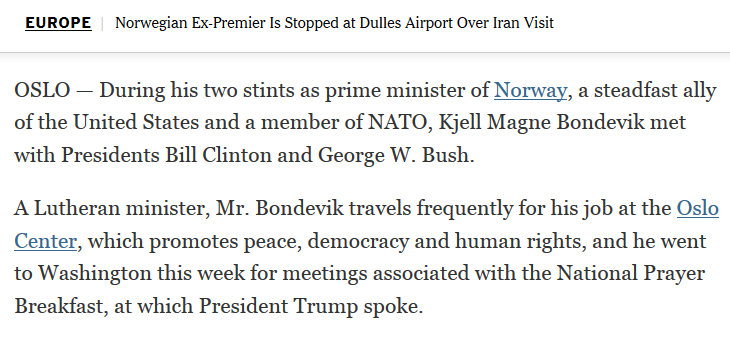
\includegraphics[width=\textwidth]{dateline.png} 
				\caption{Dateline toponym example, \textit{Source: nytimes Feb 4, 2017.}}
			\end{figure}
		\end{column}
		
	\end{columns}
	
	\vfill
} % END OF FRAME
%----------------------------------------

\subsection{Adaptive Context Features}
\frame{
	\frametitle{Adaptive \textbf{Context} Features}
	
	\begin{block}{\textbf{Context} of a toponym t}
	the other toponyms in the \textbf{window around toponym t}
	\end{block}

	\begin{overprint}
		\onslide<1>
		\begin{figure}
			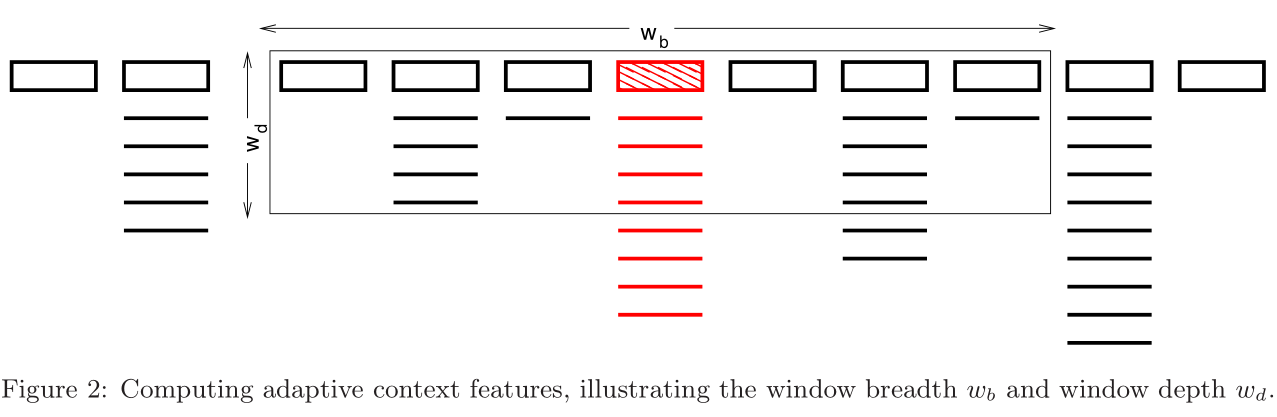
\includegraphics[width=\textwidth]{adaptive.png} 
			\caption{from Lieberman and Samet, \textit{Source: URL}}
		\end{figure}
					
	\end{overprint}

} % END OF FRAME
%----------------------------------------

\frame{
	\frametitle{\textbf{Adaptive} Context Features}
	
	\begin{block}{\textbf{Adaptive}}
		the window's \textbf{breadth $w_b$} and \textbf{depth $w_d$} can be changed
	\end{block}
	
	%\begin{block}{Depth $w_d$ of window}
	%	the number of interpretations to consider for each toponym in the window
	%\end{block}
	
	\begin{overprint}
		\onslide<1>
		\begin{figure}
			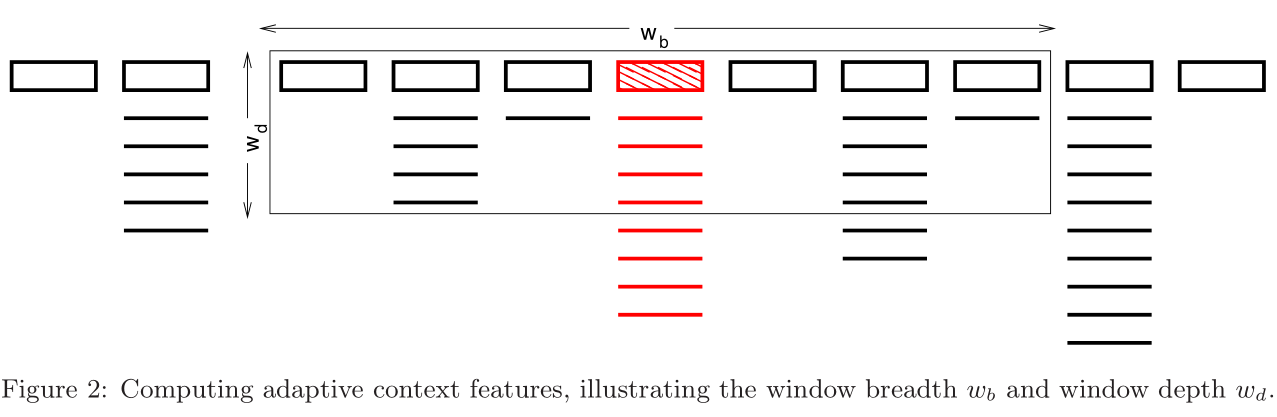
\includegraphics[width=\textwidth]{adaptive.png} 
			\caption{from Lieberman and Samet, \textit{Source: URL}}
		\end{figure}
		
		\onslide<2>
		\begin{figure}
			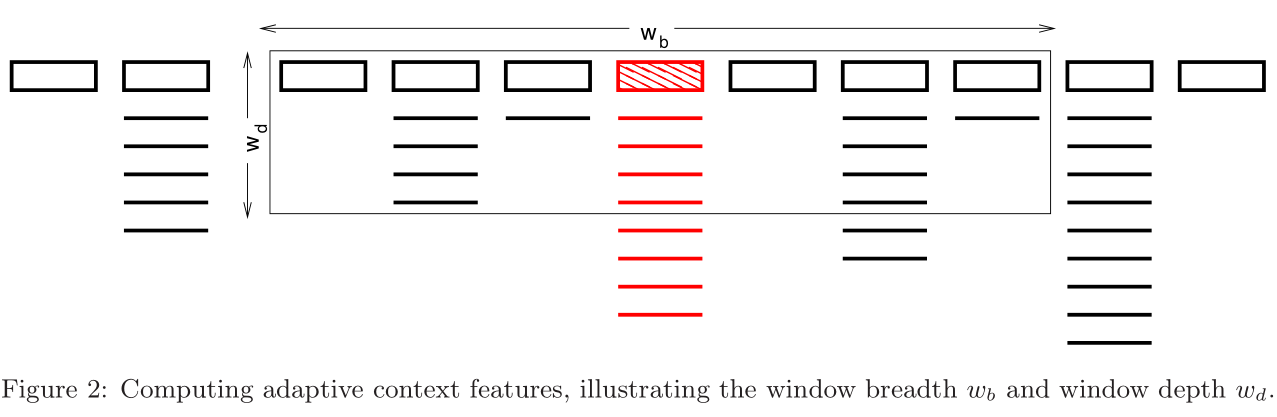
\includegraphics[width=\textwidth]{adaptive.png} 
			\caption{from Lieberman and Samet, \textit{Source: URL}}
		\end{figure}
		
		\vspace*{-5cm}
		\begin{block}{\centering advantage of adaptiveness}
			\centering {$w_b$ and $w_d$ can be changed to make the resolution process faster or more accurate!}
		\end{block}
		
	\end{overprint}
	
} % END OF FRAME
%----------------------------------------

\subsection{1. Proxmity Features}
\frame{
	\frametitle{1. Proximity Features}
	
	\begin{block}{1. Proximity Features}
		represent the average distance of an interpretation $l_t$ of toponym $t$, to the geographically closest interpretations, say $l_o$ of all the other toponyms $o$ in the window.
	\end{block}
		\begin{overprint}
		\onslide<1>
		\begin{figure}
			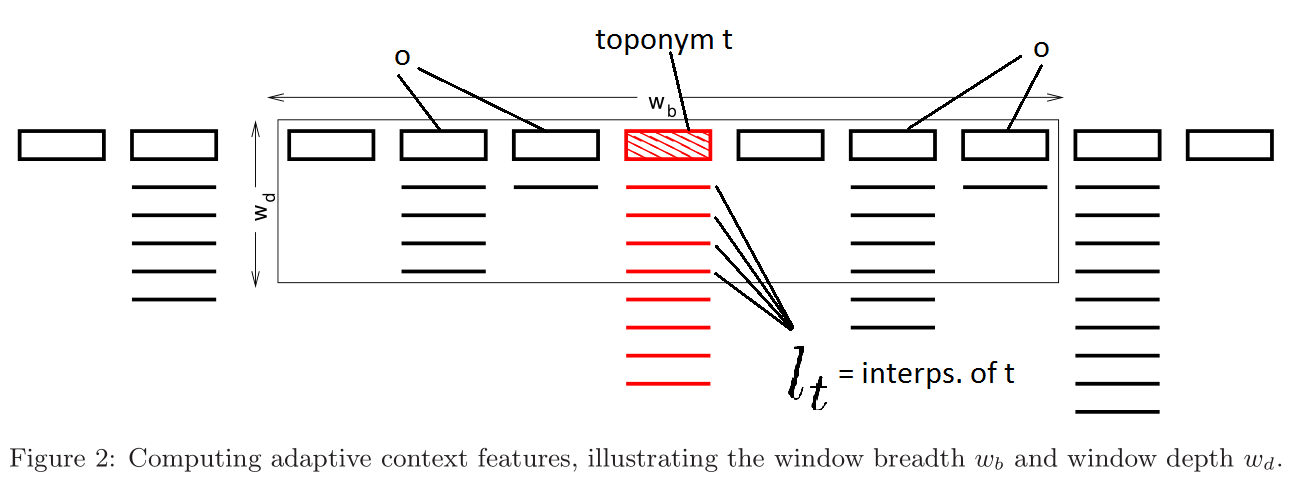
\includegraphics[width=\textwidth]{adaptive-proximity-0.png} 
			\caption{from Lieberman and Samet, \textit{Source: URL}}
		\end{figure}
		
		
	\end{overprint}
} % END OF FRAME
%----------------------------------------

\subsection{Computing Proximity Features}
\frame{
	\frametitle{Computing Proximity Features}
	
	\begin{overprint}
		\onslide<1>
		\begin{figure}
			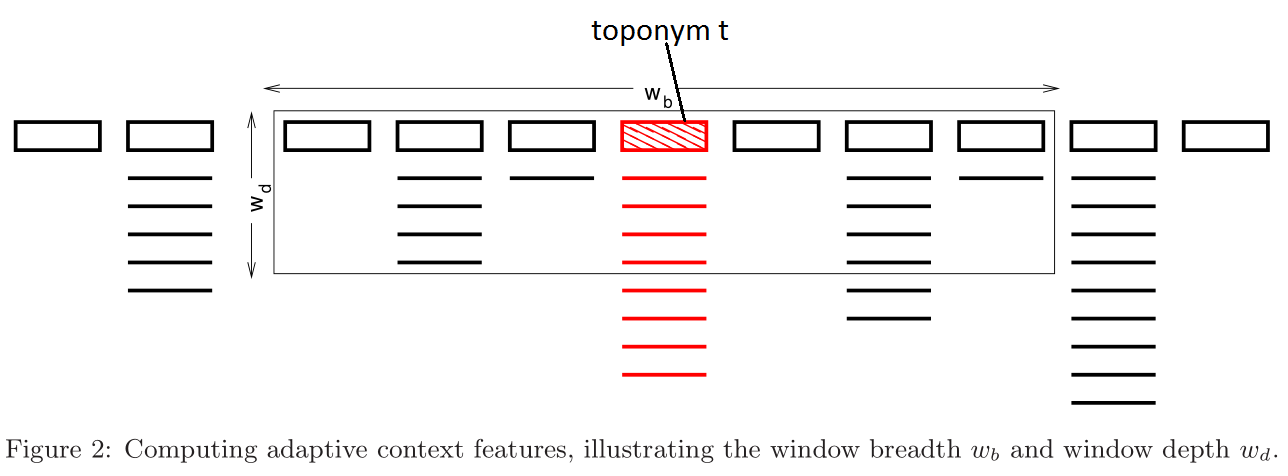
\includegraphics[width=\textwidth]{adaptive-proximity.png} 
			\caption{from Lieberman and Samet, \textit{Source: URL}}
		\end{figure}
		
		\onslide<2>
		\begin{figure}
			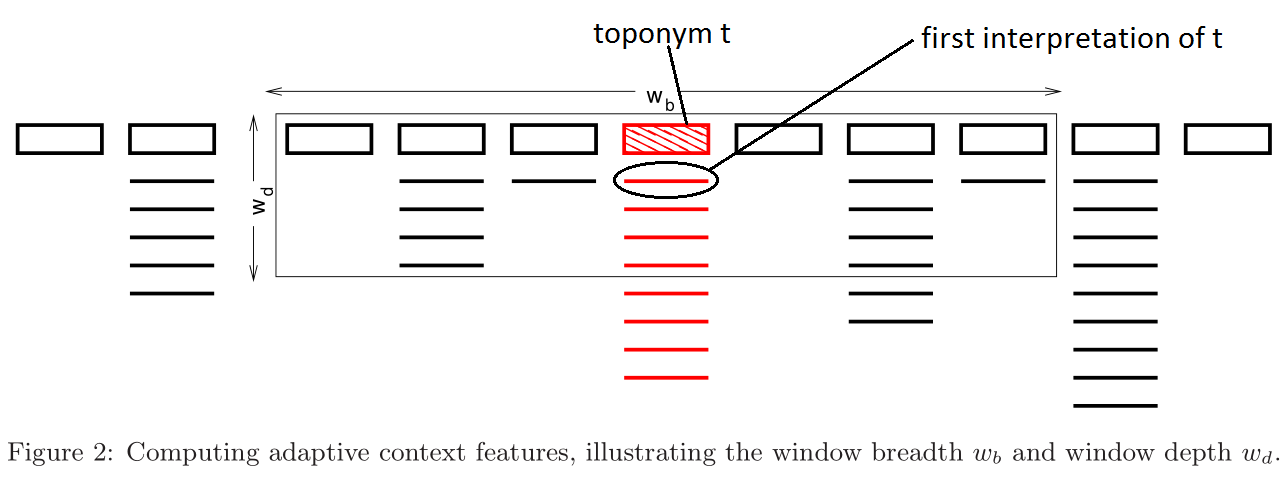
\includegraphics[width=\textwidth]{adaptive-proximity-a.png} 
			\caption{from Lieberman and Samet, \textit{Source: URL}}
		\end{figure}
		
		\onslide<3>
		\begin{figure}
			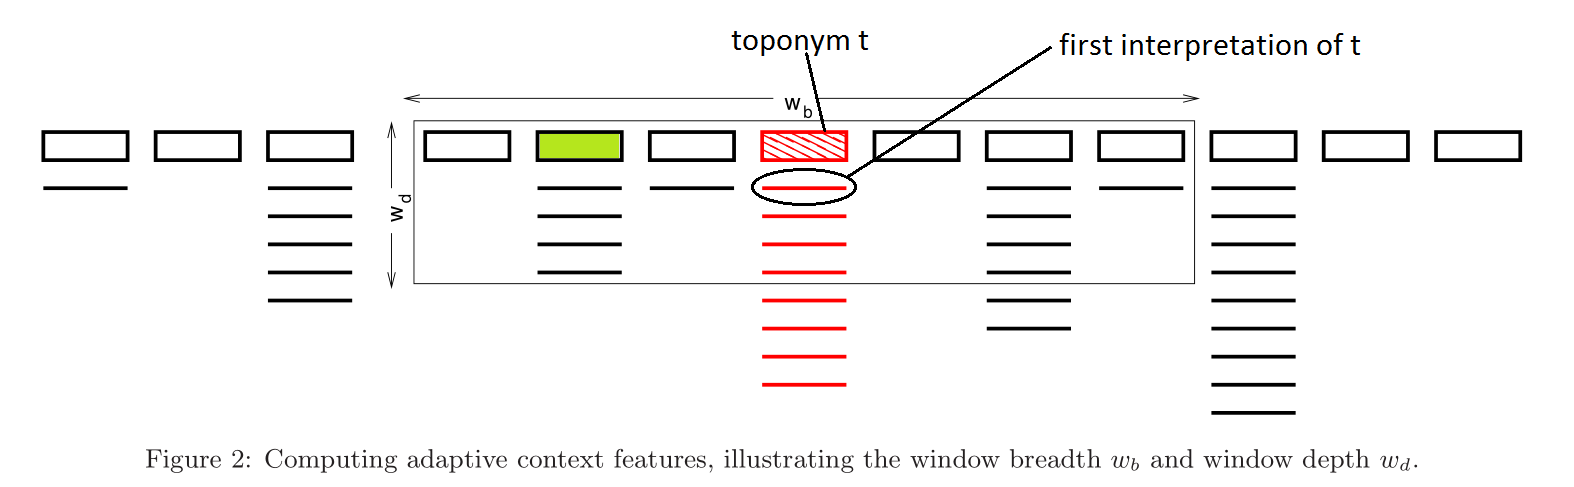
\includegraphics[width=\textwidth]{adaptive-proximity-b.png} 
			\caption{from Lieberman and Samet, \textit{Source: URL}}
		\end{figure}
		
		\onslide<4>
		\begin{figure}
			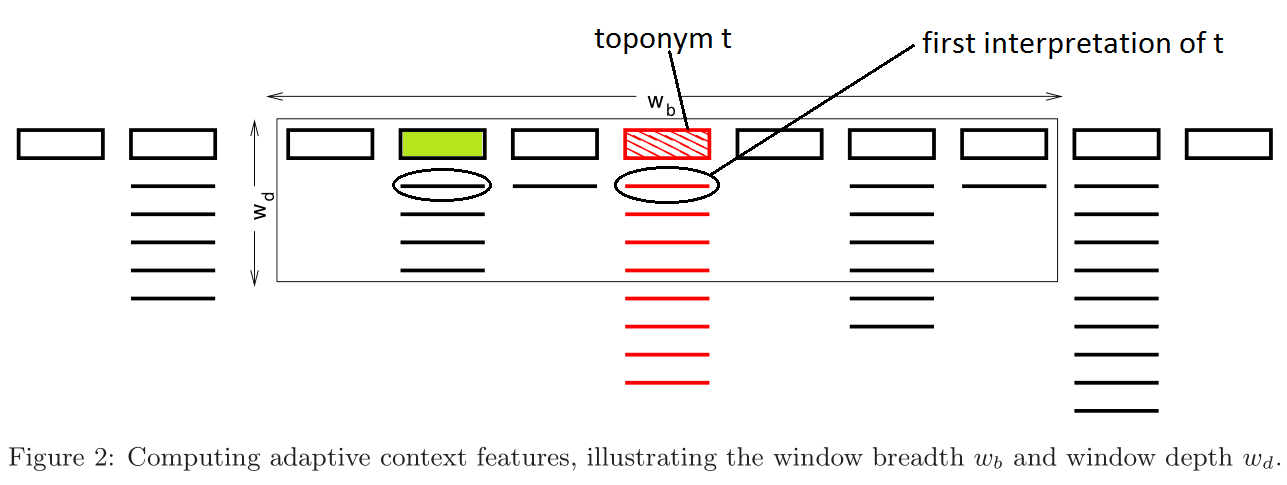
\includegraphics[width=\textwidth]{adaptive-proximity-c.png} 
			\caption{from Lieberman and Samet, \textit{Source: URL}}
		\end{figure}
		
		\onslide<5>
		\begin{figure}
			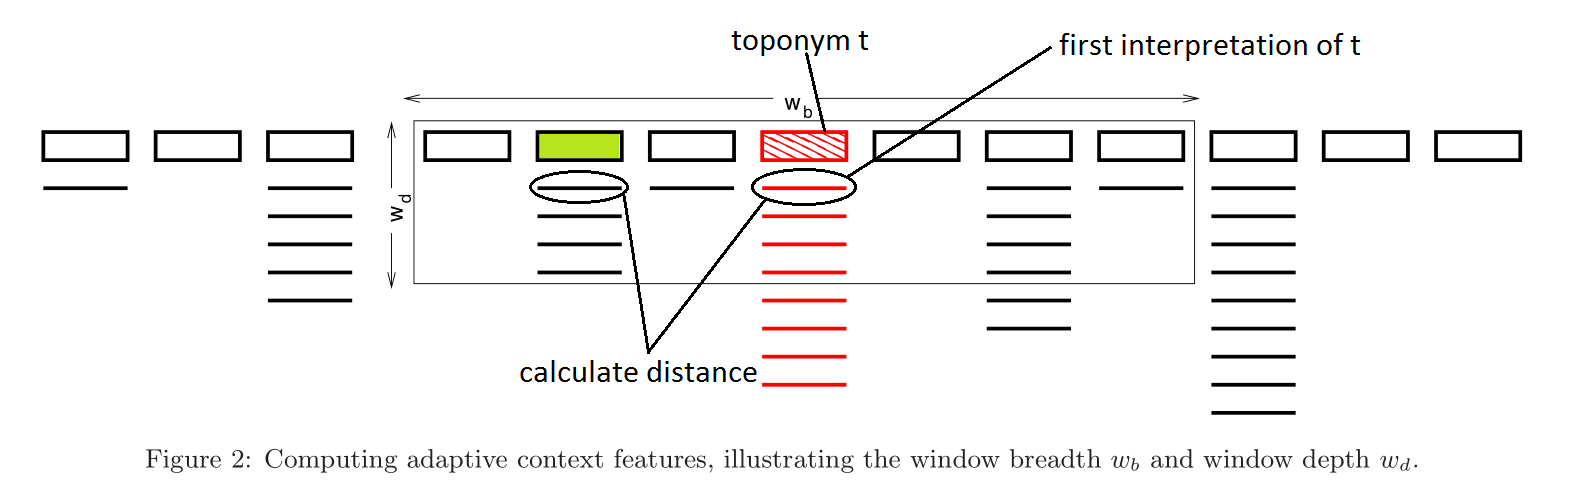
\includegraphics[width=\textwidth]{adaptive-proximity-d.png} 
			\caption{from Lieberman and Samet, \textit{Source: URL}}
		\end{figure}
		
		\onslide<6>		
		\begin{figure}
			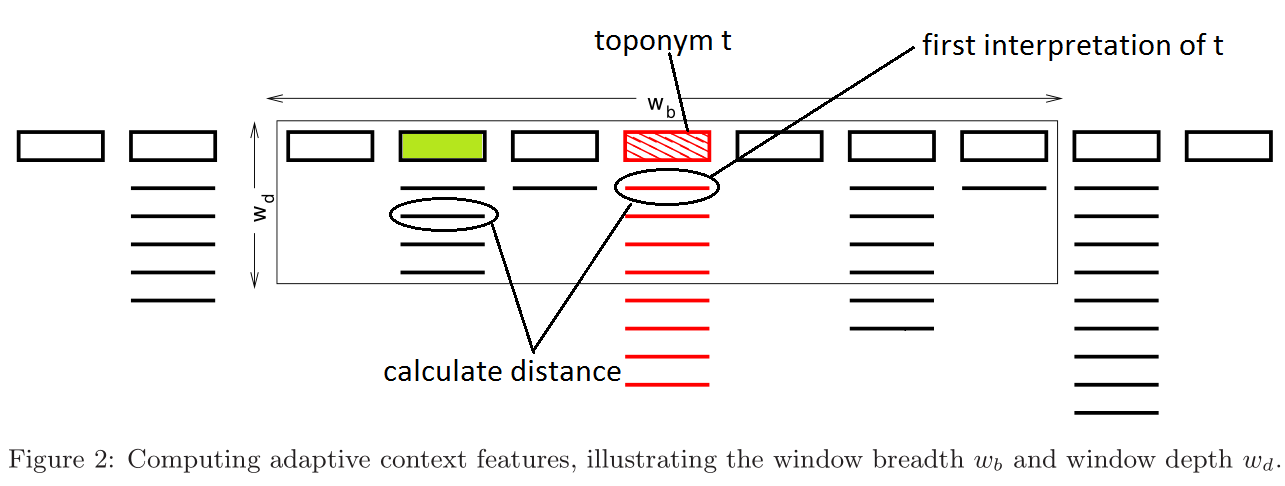
\includegraphics[width=\textwidth]{adaptive-proximity-e.png} 
			\caption{from Lieberman and Samet, \textit{Source: URL}}
		\end{figure}
		
		\onslide<7>
		\begin{figure}
			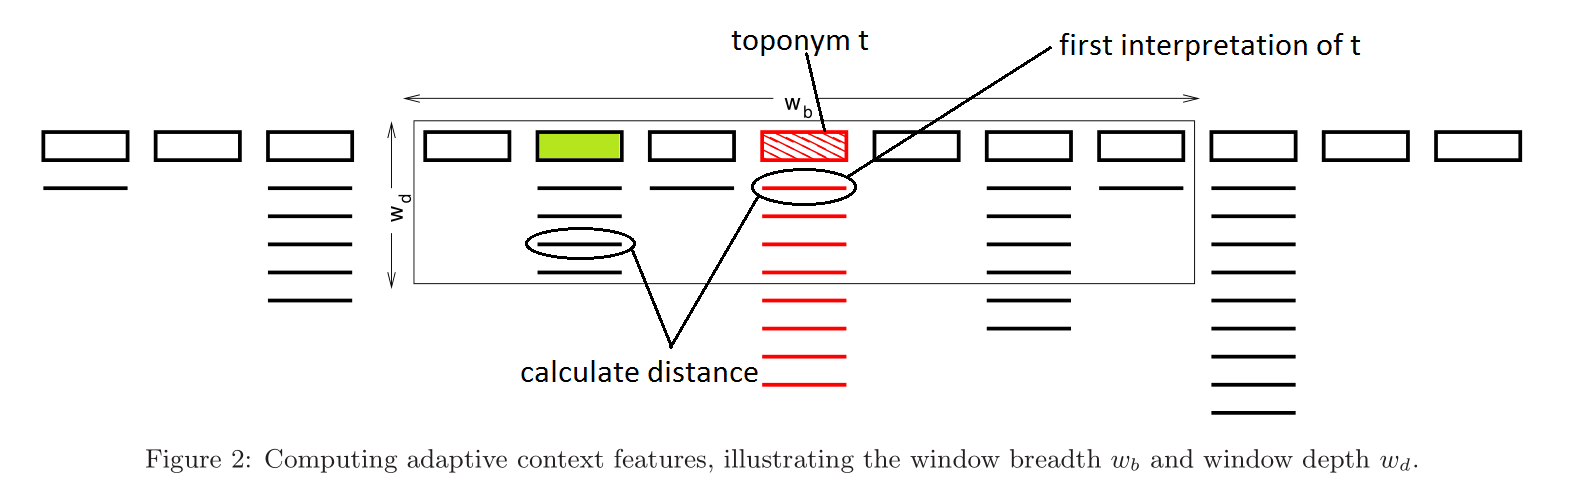
\includegraphics[width=\textwidth]{adaptive-proximity-f.png} 
			\caption{from Lieberman and Samet, \textit{Source: URL}}
		\end{figure}
		
		\onslide<8>
		\begin{figure}
			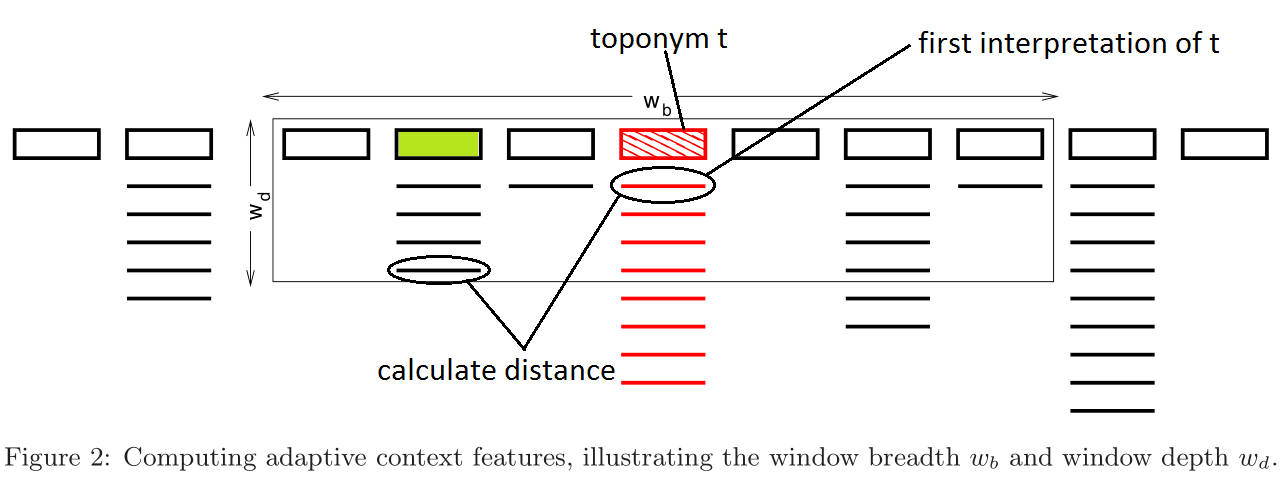
\includegraphics[width=\textwidth]{adaptive-proximity-g.png} 
			\caption{from Lieberman and Samet, \textit{Source: URL}}
		\end{figure}
		
		\onslide<9>
		\begin{figure}
			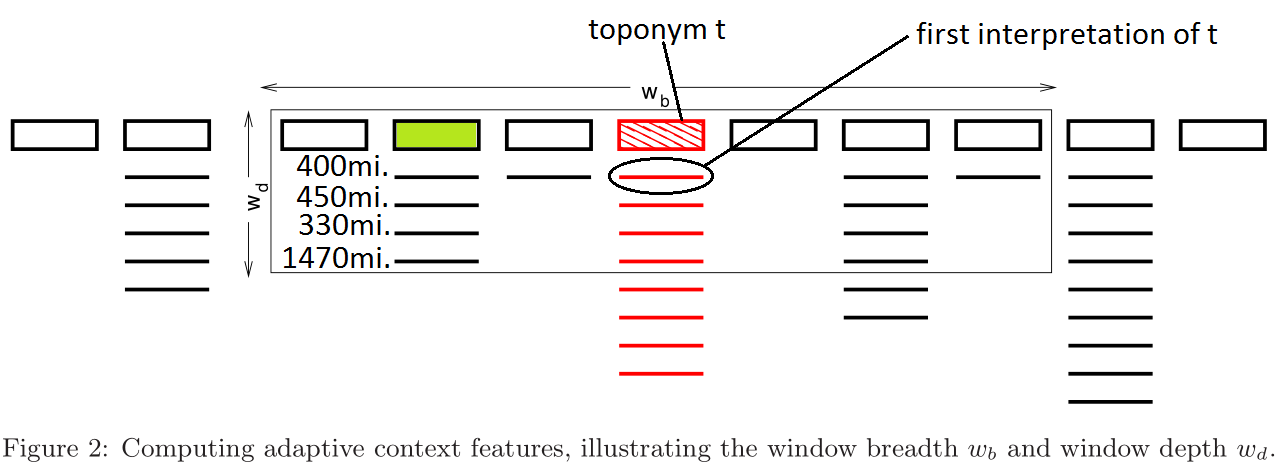
\includegraphics[width=\textwidth]{adaptive-proximity-h.png} 
			\caption{from Lieberman and Samet, \textit{Source: URL}}
		\end{figure}
		
		\onslide<10>
		\begin{figure}
			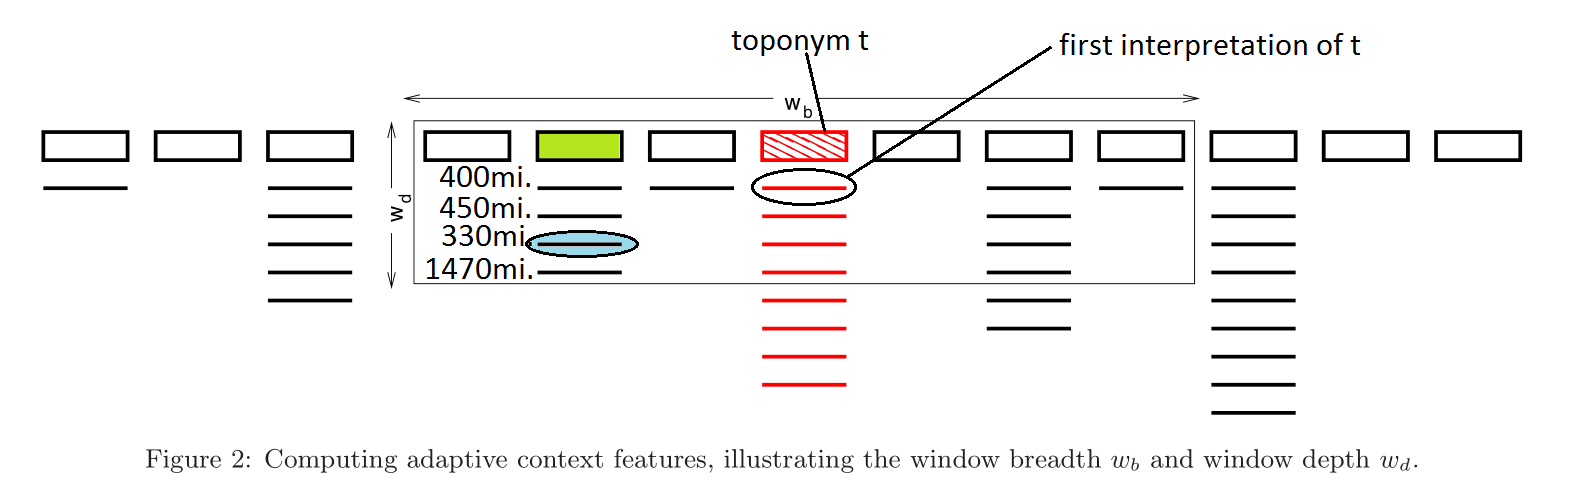
\includegraphics[width=\textwidth]{adaptive-proximity-i.png} 
			\caption{from Lieberman and Samet, \textit{Source: URL}}
		\end{figure}
		
		\onslide<11>
		\begin{figure}
			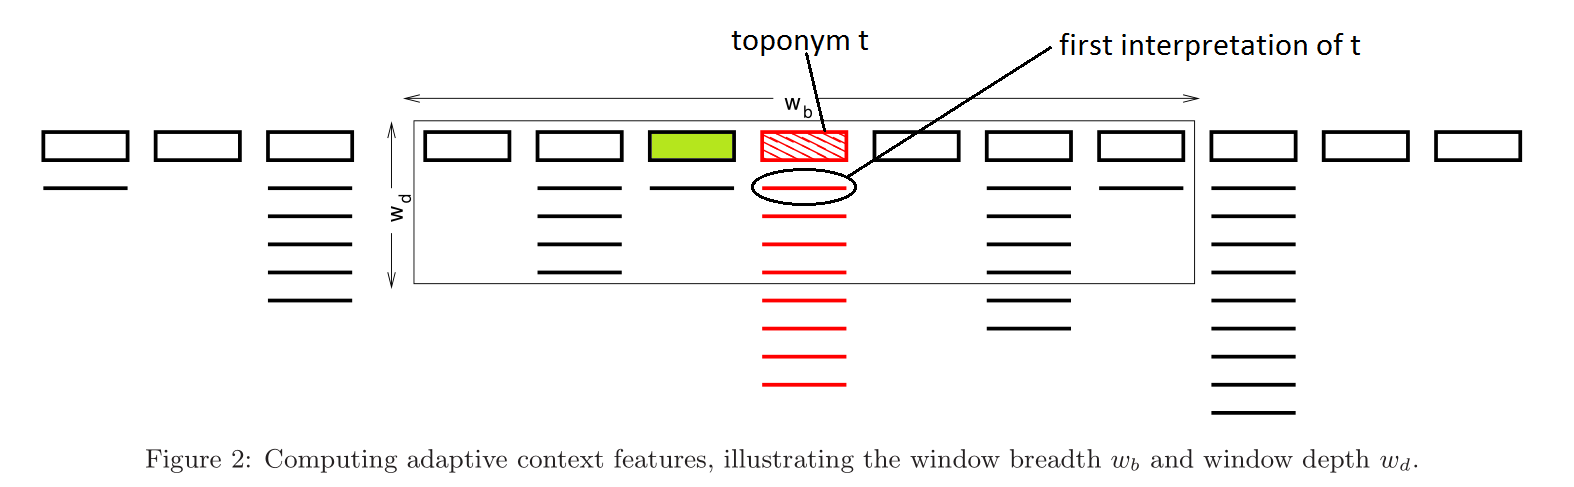
\includegraphics[width=\textwidth]{adaptive-proximity-j.png} 
			\caption{from Lieberman and Samet, \textit{Source: URL}}
		\end{figure}
		
		\onslide<12>
		\begin{figure}
			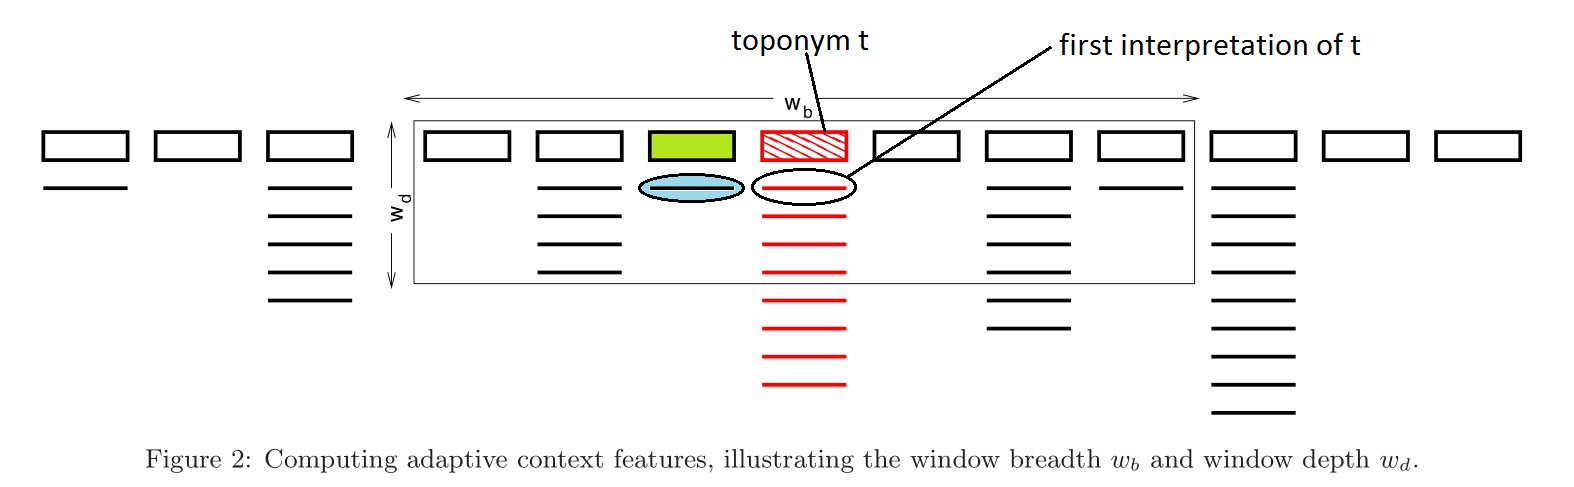
\includegraphics[width=\textwidth]{adaptive-proximity-j1.png} 
			\caption{from Lieberman and Samet, \textit{Source: URL}}
		\end{figure}
		
		\onslide<13>
		\begin{figure}
			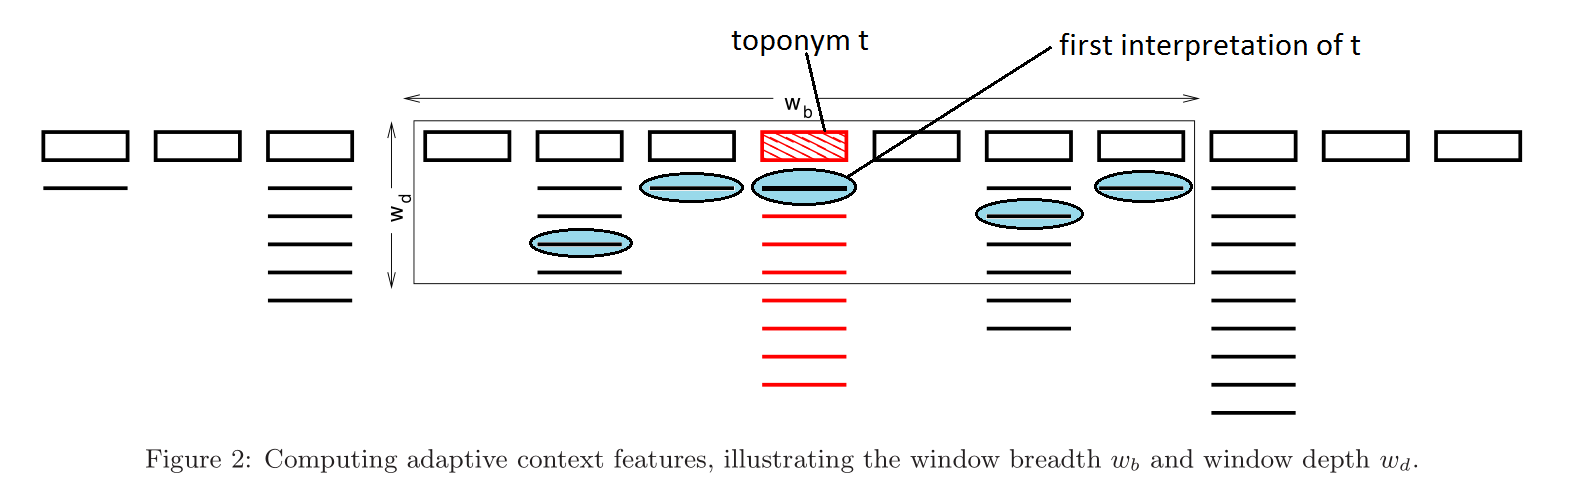
\includegraphics[width=\textwidth]{adaptive-proximity-k.png} 
			\caption{from Lieberman and Samet, \textit{Source: URL}}
		\end{figure}
		
		\onslide<14>
		\begin{figure}
			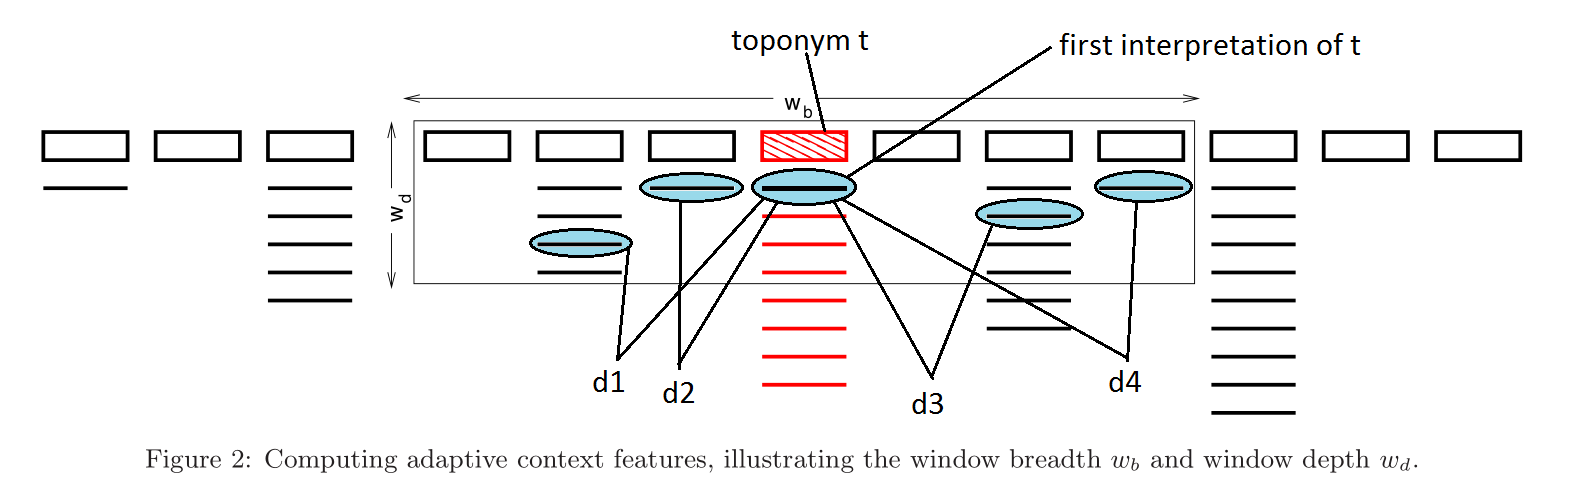
\includegraphics[width=\textwidth]{adaptive-proximity-k1.png} 
			\caption{from Lieberman and Samet, \textit{Source: URL}}
		\end{figure}
		
		\onslide<15>
		\begin{figure}
			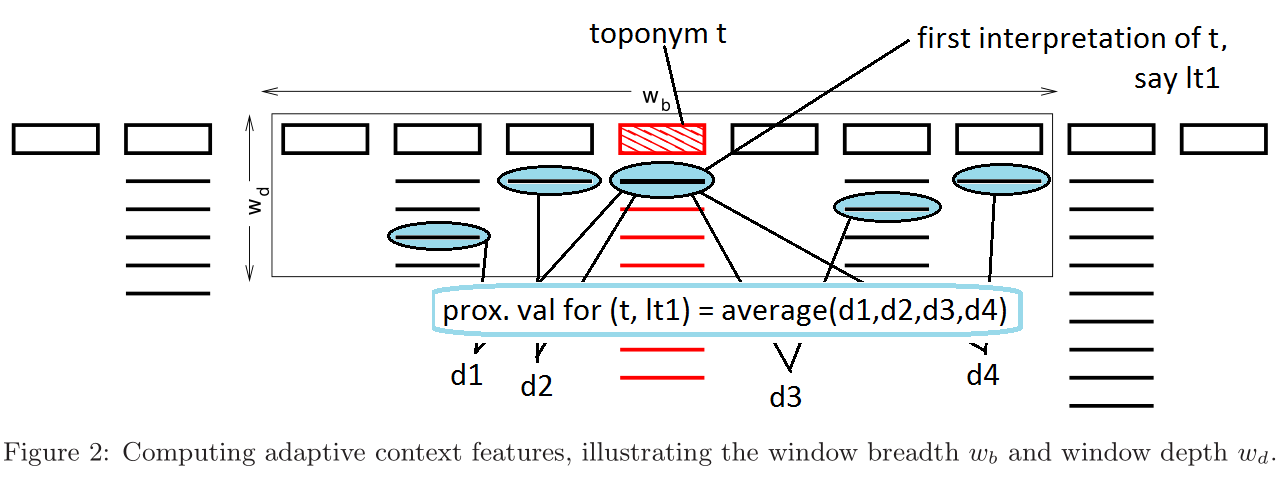
\includegraphics[width=\textwidth]{adaptive-proximity-k2.png} 
			\caption{from Lieberman and Samet, \textit{Source: URL}}
		\end{figure}
		
		\onslide<16>
		\begin{figure}
			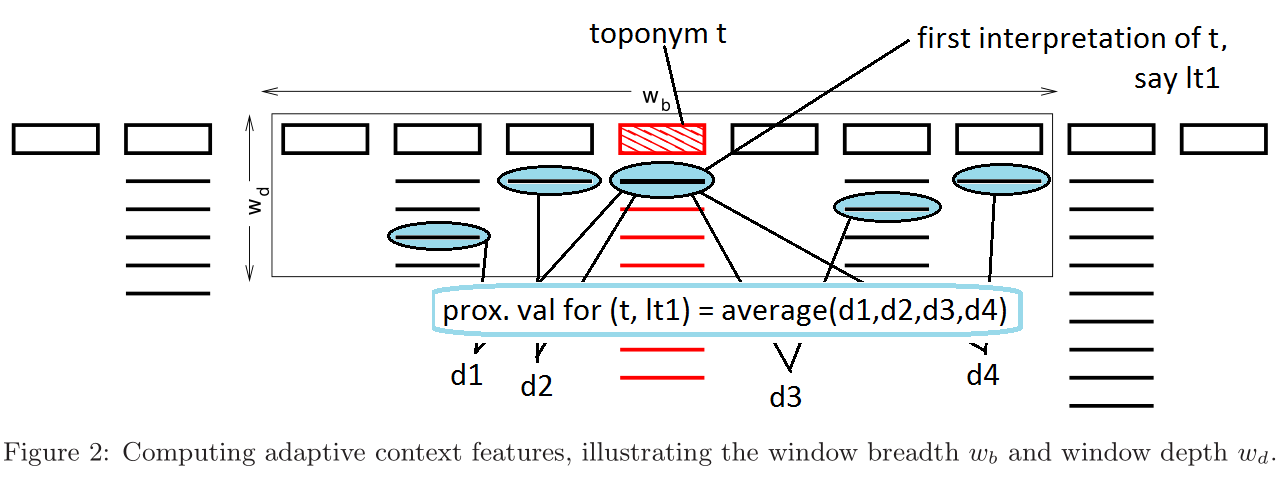
\includegraphics[width=\textwidth]{adaptive-proximity-k2.png} 
			\caption{from Lieberman and Samet, \textit{Source: URL}}
		\end{figure}
				
		\vspace*{-5cm}
		\begin{block}{\centering Proximity features}
			\centering  \textbf{the interpretation $l_t$, for which proximity score is lowest, is the chosen as the correct interpretation of $t$}
		\end{block}
		
	\end{overprint}
} % END OF FRAME
%----------------------------------------

\subsection{Proximity Features idea}
\frame{
	\frametitle{Proximity Features idea}
	
\begin{block}{\centering Proximity features}
	\centering  \textbf{all toponyms $o$ in the window around $t$ play a role in determining correct interpretation $l_t$ of $t$}
\end{block}

\pause

\begin{block}{\centering News articles}
	\centering  \textbf{generally talk about a specific region, so a news article will have many proximate toponyms}
\end{block}

	
} % END OF FRAME

%----------------------------------------

\frame{
	\frametitle{Proximity Features - example}
	
	``...,	Birmingham and Perth. It was relatively warm in London ...''
	
	\pause
	
	Assuming $w_d$=2, 
	
		\begin{tabular}{ c| c | c | c}
		{} & Birmingham & \textbf{Perth} & London \\
		\hline
		1 & UK & Scotland & UK \\
		2 & Michigan, USA & Australia & Ontario, Canada \\
		\end{tabular}
	
	\pause
	
		\begin{tabular}{c l l}
		$\checkmark$ & (Perth, Scotland) $\xrightarrow{distance}$ (Birmingham, UK) & 338.8 miles\\
		{} & (Perth, Scotland) $\xrightarrow{distance}$ (Birmingham, Michigan) & 3496.2 miles \\
		\pause
		$\checkmark$ & (Perth, Scotland) $\xrightarrow{distance}$ (London, UK) & 450.6 miles \\
		{} & (Perth, Scotland) $\xrightarrow{distance}$ (London, Ontario) & 3403.7 miles \\
		\end{tabular} \\
		
		... \\
		\pause
		prox score(Perth, Scotland) = average(338.8, 450.6) = 394.7\footnotemark miles \\
				
	\only<2->{\footnotetext[1]{The authors used geometric median for average}}
		
	\vfill
} % END OF FRAME

%----------------------------------------
\subsection{Proximity Features - example}
\frame{
	\frametitle{Proximity Features - example}
	
	``...,	Birmingham and Perth. It was relatively warm in London ...''
	
	\pause
	
	Assuming $w_d$=2, 
	
	\begin{tabular}{ c| c | c | c}
	{} & Birmingham & \textbf{Perth} & London \\
	\hline
	1 & UK & Scotland & UK \\
	2 & Michigan, USA & Australia & Ontario, Canada \\
	\end{tabular}
	
	\pause
	
	prox score(Perth, Scotland) = average(338.8, 450.6) = 394.7\footnotemark[1] miles  \\
	
	\pause
	
	similarly we calculate prox score for second $(t, l_t)$ pair  \\
	
	
	\begin{tabular}{c l l}
	$\checkmark$ & (Perth, Australia) $\xrightarrow{distance}$ (Birmingham, UK) & 9085 miles\\
	{} & (Perth, Australia) $\xrightarrow{distance}$ (Birmingham, Michigan) & 11,175 miles \\
	$\checkmark$ & (Perth, Australia) $\xrightarrow{distance}$ (London, UK) & 9007 miles \\
	{} & (Perth, Australia) $\xrightarrow{distance}$ (London, Ontario) & 11,245 miles \\
	\end{tabular} \\
	
	
	
	\pause
	
	prox score(Perth, Australia) = average(9085, 9007) = 9046\footnotemark[1] miles  \\
	
	\pause
	
	\begin{overprint}
		\vspace*{-3cm}
		\begin{block}{\centering Proximity features}
			\centering So the \textbf{correct interp.} for Perth, in this context, using Prox feature only would be \textbf{(Perth, Scotland)}! \\
			\centering as prox score(Perth, Scotland) \textless prox score(Perth, Australia)
		\end{block}
	\end{overprint}
	
	

	
	
	\only<2->{\footnotetext[1]{The authors used geometric median for average}}
	

	\vfill
} % END OF FRAME
%----------------------------------------


\subsection{2. Sibling Features}
\frame{
	\frametitle{2. Sibling Features}
	
	\begin{block}{2. Sibling Features}
		capture the toponyms that belong to same country, state	or any other administrative division
	\end{block}
	
	\pause
	
	\begin{itemize}
		\item capture sibling relations
		\item capture containment relationships 
	\end{itemize}
	
	\pause
	
	e.g. ``Saarbruecken and Voelklingen" are siblings at city level \\
	
	\pause
	
	e.g. "Paris, Texas" refers to Paris in Texas, USA \\
	
	\pause
	
	\textbf{computed in a similar way as the proximity features!}
	
} % END OF FRAME
%----------------------------------------

\subsection{Sibling Features idea}
\frame{
	\frametitle{Sibling Features idea}
	
	\begin{block}{\centering Sibling features}
		\centering  determine \textbf{correct interpretation} for toponyms that are \textbf{geographically not proximate} but have \textbf{common parent} such as state or country
	\end{block}
	
%	\pause
	
%	\begin{block}{\centering Sibling features}
%		\centering  \textbf{can correctly capture relationships which may be considered geographically distant}
%	\end{block}
	
	\vfill
} % END OF FRAME
%----------------------------------------

\subsection{Sibling Features - example}
\frame{
	\frametitle{Sibling Features - example}
	
	``... Bloomington, Rochester and Duluth. ..."
	
	\pause
	
	Assuming $w_d$=3, 
	
	\begin{tabular}{ c| c | c | c}
		
		{} & Bloomington & \textbf{Rochester} & Duluth \\
		\hline
		1 & Minnesota, USA & Victoria, Australia & Georgia, USA\\
		2 & Michigan, USA & New York, USA & Minnesota, USA\\
		3 & {} & Minnesota, USA & {}\\
	\end{tabular} \\
	
	... \\
	\pause
	
	
	\textbf{The sibling feature scores for toponym/interp pairs will be}
	\begin{tabular}{ c| c | c | c}
		
		{} & $(t, l_t)$ & Score & common sibling levels. \\
		\hline
		1 & (Rochester, Victoria Australia) & 0 & -\\
		\pause
		2 & (Rochester, New York USA) & 4 & 4 x USA\\
		\pause
		3 & (Rochester, Minnesota USA) & 6 & 4 x USA, 2 x Minnesota\\
	\end{tabular}
	
	\pause
	
	\begin{overprint}
		\vspace*{-2.5cm}
		\begin{block}{\centering Sibling features}
			\centering \textbf{correct interp.} = \textbf{(Rochester, Minenesota)}! \\
			\centering as sibling score(Rochester, Minnesota) is \textbf{largest} among all toponym/interp pairs!
		\end{block}
	\end{overprint}
	
	\vfill
} % END OF FRAME
%----------------------------------------

\subsection{interpretations order}
\frame{
	\frametitle{interpretations order}
	
	``... Bloomington, Rochester and Duluth. ..."
	
	\pause
	
	Assuming \textbf{$w_d$=2}, 
	
	\begin{tabular}{ c| c | c | c}
		
		{} & Bloomington & \textbf{Rochester} & Duluth \\
		\hline
		1 & Minnesota, USA & Victoria, Australia & Georgia, USA\\
		2 & Michigan, USA & New York, USA & Minnesota, USA\\
	\end{tabular} \\
	
	... \\
	\pause
	
	
	\textbf{The sibling feature scores for toponym/interp pairs will be}
	\begin{tabular}{ c| c | c | c}
		
		{} & $(t, l_t)$ & Score & common sibling levels. \\
		\hline
		1 & (Rochester, Victoria Australia) & 0 & -\\
		\pause
		2 & (Rochester, New York USA) & 4 & 4 x USA\\
	\end{tabular}

	\vfill
} % END OF FRAME
%----------------------------------------

%\subsection{feature propagation}
%\frame{
%	\frametitle{feature propagation}
%	
%	\begin{itemize}
%		\item toponym t considered once in window
%		\item feature propagation - after toponym resolution
%	\end{itemize}
%	
%	\vfill
%} % END OF FRAME
%----------------------------------------
\subsection{Evaluation measures}
\frame{
	\frametitle{Evaluation measures}
	
	\begin{itemize}
		\item Precision
		\item Recall
		\item F1 score
	\end{itemize}
	
	\pause

	Precision = $\frac{\text{no. of correctly resolved toponyms}}{\text{no. of total resolved toponyms}}$ \\
	...\\
	Recall = $\frac{\text{no. of correctly resolved toponyms}}{\text{no. of true toponyms}}$

	\vfill
} % END OF FRAME
%----------------------------------------


\subsection{Evaluation results}
\frame{
	\frametitle{Evaluation results}
	
	\begin{itemize}
		\item  news data from ACE, LGL and CLUST datasets
		\item  compared with two commercial geotagging frameworks i.e. (Thomson Reuter's OpenCalais and Yahoo!'s Placemaker)
	\end{itemize}
	
	\pause
	
	\textbf{performed better in majority of test scenarios and datasets} \\
	
	(details in the original paper)
	
} % END OF FRAME
%----------------------------------------


%========================================
%========================================

\section[Applications]{Applications}

%\subsection{Highlighting}

%----------------------------------------

\def\hilite<#1>{%
	\temporal<#1>{\color{black}}{\color{MPIIred}}%
	{\color{gray}}}

%----------------------------------------

%\subsection{Geographic visualization and browsing}
%\frame{
%	\frametitle{Geographic visualization and browsing}
%	
%	\begin{itemize}
%		\item thematic maps
%		\item geographic anchoring of encyclopedia articles
%	\end{itemize}
%		
%} % END OF FRAME

%----------------------------------------

\subsection{Question answering}
\frame{
	\frametitle{Question answering}
	
	trend in search engines to \textbf{answer some queries directly}, instead of returning search results \\
	
	\pause
	
	e.g. consider the query ``What is the distance between between Lahore and Multan?" \\
	...\\
	
	\pause
	
	can be solved by
	\begin{itemize}
		\item (1) resolve both toponyms in the query, 
		\item (2) compute the geographic distance using a geometric formula
	\end{itemize}
	
} % END OF FRAME

%----------------------------------------

\subsection{Improving search results}
\frame{
	\frametitle{Improving search results - for geographic queries}
	
	return relevant documents which would not be returned using keyword based search only \\
	...\\
	
	\pause
	
	e.g. query is "Saarland" \\
	
	should also return documents which mention cities of Saarland, but not the keyword \textbf{Saarland} in them! \\
	...\\
	\pause
	
	can be done by assigning \textbf{geographic focus} to documents
	
} % END OF FRAME


%----------------------------------------

\subsection{Browsing news geographically}
\frame{
	\frametitle{Browsing news geographically}
	
	
	e.g. system \textbf{NewsStand System: }	
	users can \underline{browse news geographically on world map} in  an \textbf{interactive} manner
	\pause
	\bigskip
	\begin{itemize}
		\item crawls around 50,000 news article every day
		\item cluster them on content and \textbf{location}
		\item associate each cluster to its \textbf{geographic focus}
		\item stories appear as the map as the map is zoomed in/out
	\end{itemize}
	
} % END OF FRAME

%----------------------------------------

\subsection{Browsing news geographically - NewsStand}
\frame{
	\frametitle{Browsing news geographically - NewsStand}
	
	
	\begin{overprint}
		\onslide<1>
		\begin{figure}
			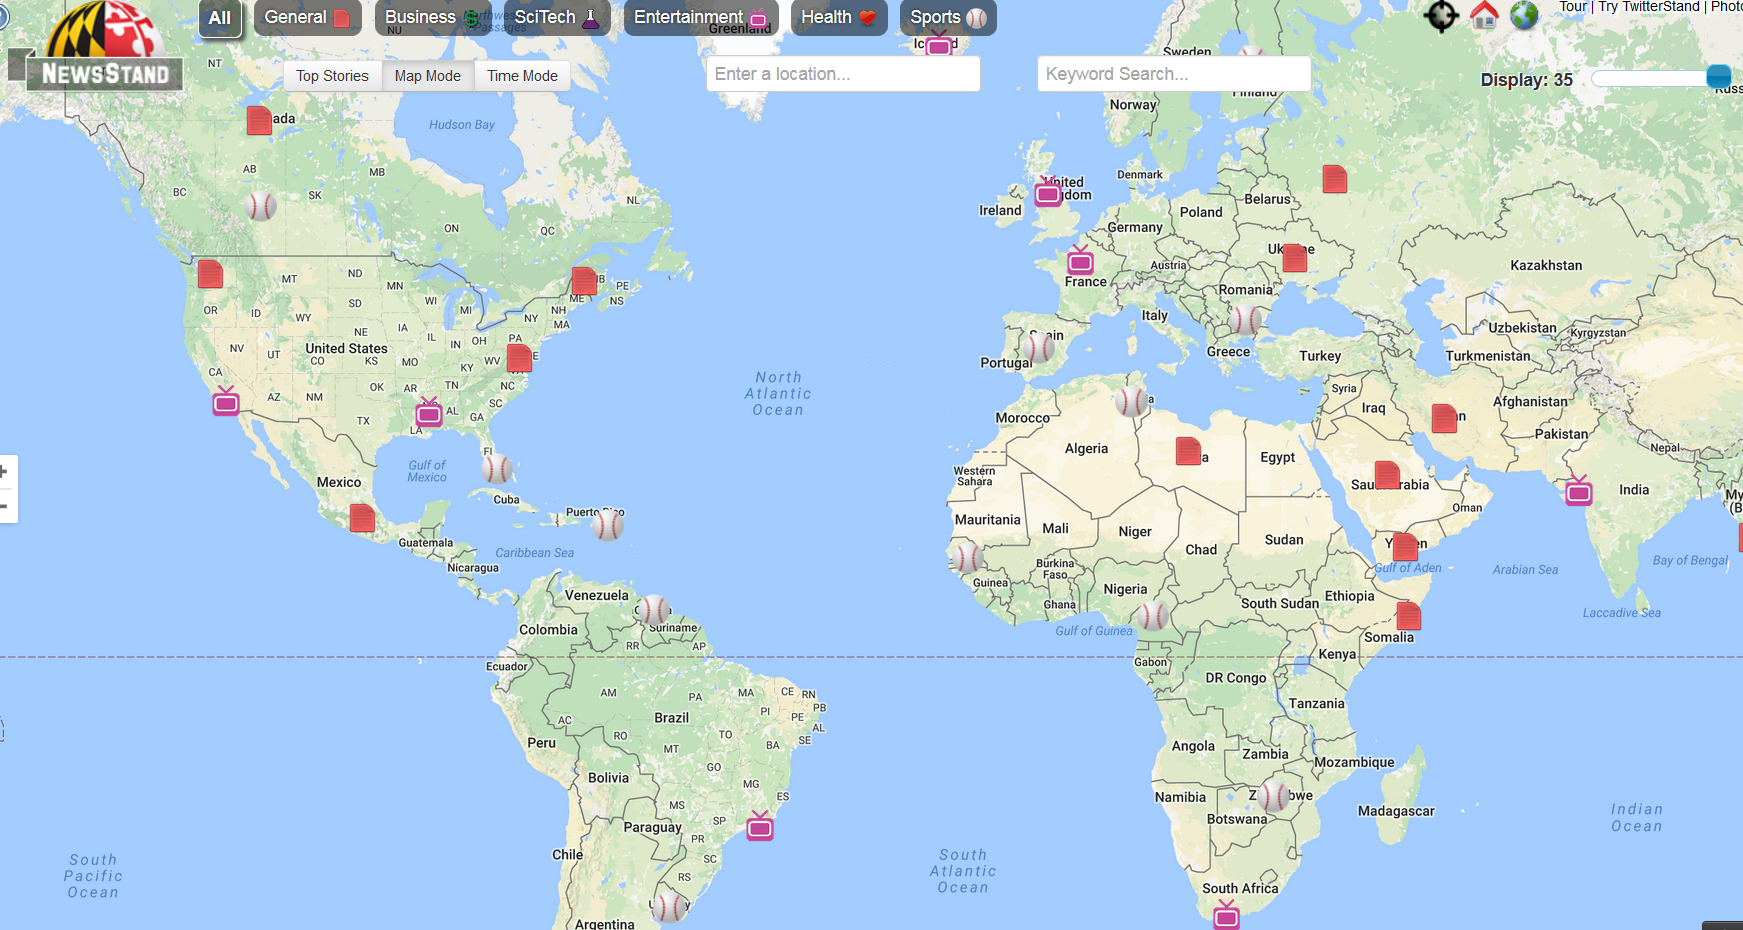
\includegraphics[width=\textwidth]{aus0.png} 
			\caption{NewsStand System, \textit{Source: URL}}
		\end{figure}
		
		\onslide<2>
		\begin{figure}
			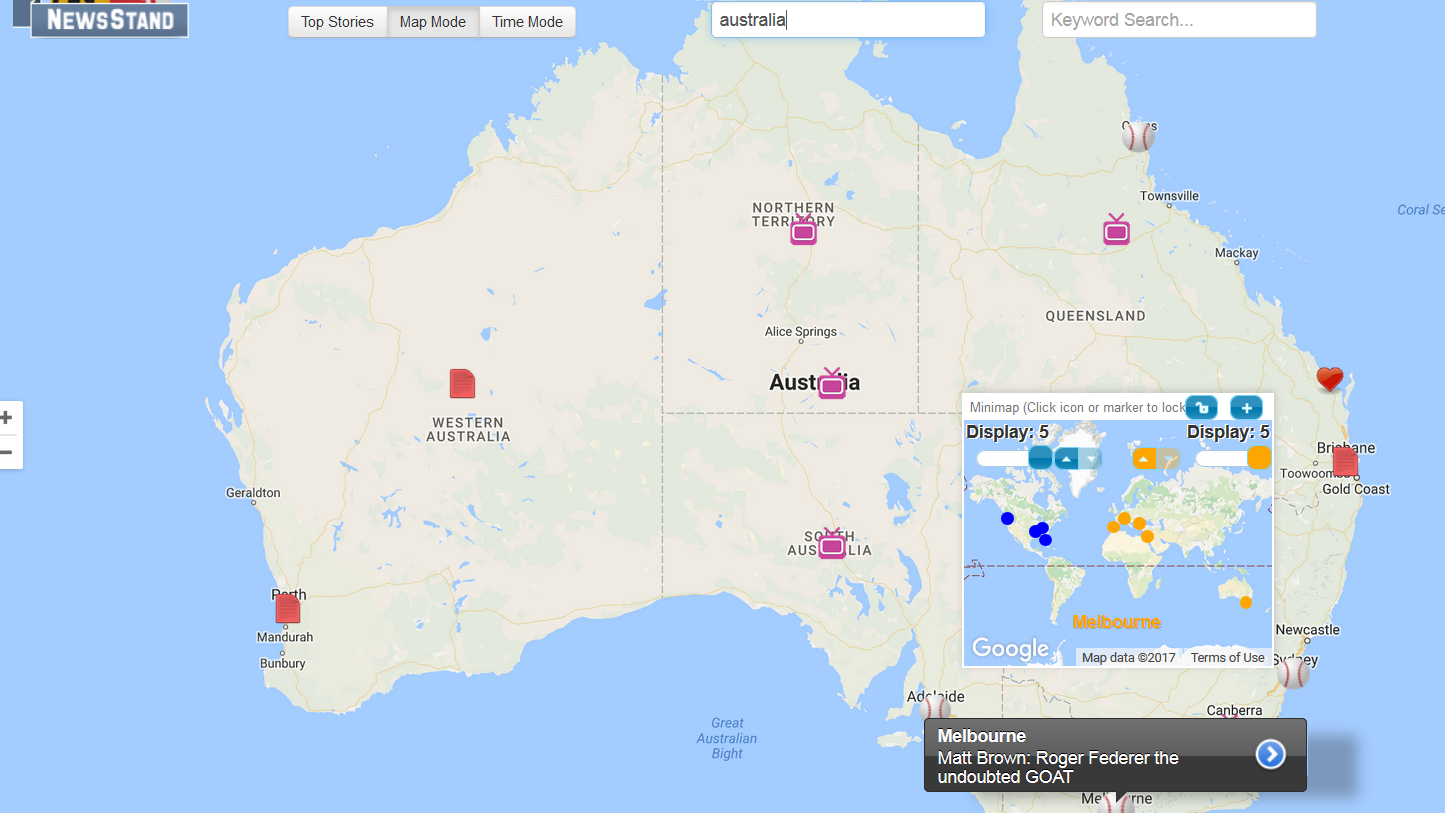
\includegraphics[width=\textwidth]{aus1.png} 
			\caption{NewsStand System, \textit{Source: URL}}
		\end{figure}
		
		\onslide<3>
		\begin{figure}
			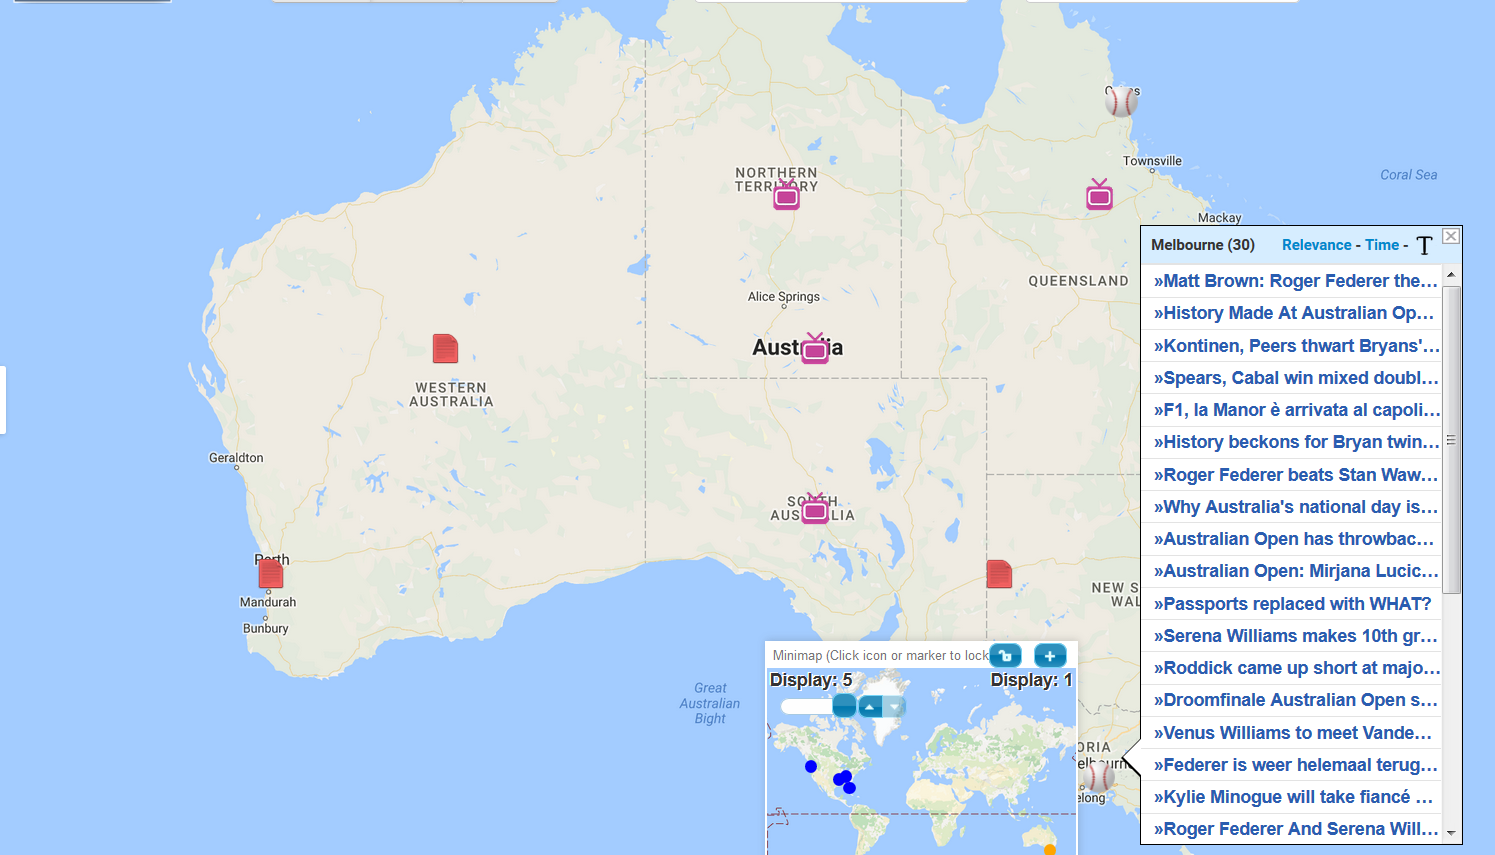
\includegraphics[width=\textwidth]{aus2.png} 
			\caption{NewsStand System, \textit{Source: URL}}
		\end{figure}
	\end{overprint}
	
	\vfill
} % END OF FRAME
%========================================
%========================================



\section[Conclusion]{Conclusion}
\subsection{Conclusion}
\frame{
	\frametitle{Conclusion}
	
	\begin{itemize}
		\item Toponyms
		\item Geotagging
		\begin{itemize}
			\item Toponym recognition
			\item Toponym resolution
		\end{itemize}
		\item Context free features
		\item Adaptive context features
		\item Geotagging has many applications/usecases
	\end{itemize}
		
} % END OF FRAME


%----------------------------------------
\subsection{Questions}
\frame{\frametitle{Questions}

\begin{center}\begin{LARGE}\textbf{Questions?}\end{LARGE}\end{center}


}

\subsection{References}
\frame{
	\frametitle{References}

	\begin{itemize}
		\item  Michael D. Lieberman and Hanan Samet. Adaptive Context Features for Toponym Resolution in Streaming News. In In SIGIR'12: Proceedings of the 35th International ACM SIGIR Conference on Research and Development in Information Retrieval, pages 731$-$740, 2012.
		\item Jochen L Leidner. Toponym Resolution in Text : Annotation, Evaluation and Applications of Spatial Grounding of Place Names. Universal Press, Boca Raton, FL, USA, 2008.
		\item Michael D Lieberman, Hanan Samet, and Jagan Sankaranarayanan. Geotagging with local lexicons to build indexes for textually-specified
		spatial data. In 2010 IEEE 26th International Conference on Data Engineering (ICDE 2010), pages 201$-$212. IEEE, 2010.
	\end{itemize}

\vfill
}

\newcommand{\backupbegin}{
   \newcounter{framenumberappendix}
   \setcounter{framenumberappendix}{\value{framenumber}}
}
\newcommand{\backupend}{
   \addtocounter{framenumberappendix}{-\value{framenumber}}
   \addtocounter{framenumber}{\value{framenumberappendix}} 
}

\appendix
\backupbegin


\backupend

\end{document}
